\section { Computer Vision }
	\subsection { The pinhole camera model }
		Cameras project 3-dimensional scenes onto a 2-dimensional plane - the image plane.
		The overall projection of a single point in space (given in a world copordinate system) to the image plane can be divided into two independent successive operations \cite[S.~50]{Szeliski2010}:
		
		\subsubsection{Extrinsic parameters}
			A camera's extrinsic parameters describe its position and pose relative to the world coordinate system. For a simple pinhole camera those parameters are given with 
			
			\begin{equation}
			\matr{C}_{ext} = \begin{bmatrix}
						\matr{R}_{3\times 3} & T_{3\times 1}\\
						0_{1\times 3} & 1
						\end{bmatrix}_{4\times 4} = -\matr{R}^{-1}T = -\matr{R}^TT \, . 
			\end{equation}
			$\matr{R}_{3\times 3}$ is a rotation matrix that represents the camera's rotation relative to the world coordinate system and T is the position of the world coordinate system, given in the new, camera-centered coordinate system. 
	
		\subsubsection{Intrinsic parameters}
			A camera intrinsic parameters reflect its internal structure and depend on focal length $f_{2\times 1}$, size of the image sensor and the principal point $c_{2\times1}$ which is defined as the intersection of the camera's optical axis with the image plane, denoted in pixel coordinates. This point ideally corresponds with the image sensor's center but might be slightly offset because of small misalignments within the camera.
			
			All in all this results in the camera's intrinsic matrix
			\begin{equation}
			\matr{C}_{int} = \begin{bmatrix}
				f_x & s & c_x  \\
				0 & f_y & c_y \\
				0 & 0 & 1 
				\end{bmatrix}.
			\end{equation}
			The factor $s$ encodes any possible skew that might be introduced through misalignments between the camera's sensor and its optical axis and can typically be set to $0$ without affecting the approximation of the camera model too much.
		
		\subsubsection{Combined model}
			Combined, the intrinsic and extrinsic matrices lead to the camera matrix \cite{Szeliski2010}:
			
			\begin{equation}
			\matr{C} = \begin{bmatrix}\matr{C}_{int} & \matr{0}\\\matr{0}^T & 1\end{bmatrix}
			\begin{bmatrix}\matr{R} & T\\\matr{0}^T & 1\end{bmatrix}
			\end{equation}
			
			which maps a point $p_w = \left(x_w, y_w, z_w, 1\right)$ given in world coordinates to screen coordinates and disparity $d$, $p_s = \left(x_s, y_s, 1, d\right)$.
			
			Since the inputs for neural networks often have to be scaled, it is also desirable to include this fact in the equation for the projection. Assuming two parameters $a_x$ and $a_y$ for the scale factors in width and height of the image, the full projection matrix is now
			
			\begin{equation}
			\matr{C}' = \begin{bmatrix}a_x & 0 & 0 & 0\\ 0 & a_y & 0 & 0\\0 & 0 & 1 & 0\\0 & 0 & 0 & 1\end{bmatrix} \begin{bmatrix}\matr{C}_{int} & \matr{0}\\\matr{0}^T & 1\end{bmatrix}
			\begin{bmatrix}\matr{R} & T\\\matr{0}^T & 1\end{bmatrix} \,.
			\end{equation}
		
\section { Neural Networks }
	Artificial neural networks 	are modeled on the biological function of human nerve tracts. Early steps towards development and application of an artificial model of human neurons were made between 1943 and 1958 \cite{McCulloch1943, ROSENBLATT1958}. In 1958, Rosenblatt introduced the perceptron, a binary classifier mapping an input vector $\vec{x}$ to two classes, 1 and 0:
	
	\begin{equation}
	\label{eq:rosenblatt-perceptron}
	f(\vec{x}) =
	\begin{cases}
	1\text{, if } \vec{w}^{\,T}\vec{x} + b \geq 0 \\
	0\text{, else.}
	\end{cases}
	\end{equation}
	
	Depending on the weights $\vec{w}$ and the bias $b$, the perceptron can either "`fire"' (produce 1 as output) or "`not fire"' (produce 0 as output) for a given input vector $\vec{x}$. This concept is inspired by biological neurons which only fire an action potential if the amount of incoming stimuli reaches a certain threshold.
	
	Due to its linear nature, this model is not able to reliably predict the outcome of real-world processes, which are mostly non-linear by nature. In 1962, Rosenblatt was able to overcome this limitation by stacking perceptrons into layers and chaining two or more layers to create a \markup{MLP}\nomenclature{MLP}{Multilayer Perceptron} \cite{ROSENBLATT1961} as shown in Figure \ref{fig:mlp}. 
	
	\begin{figure}
					\tikzset{%
				every neuron/.style={
					circle,
					draw,
					minimum size=1cm
				},
				neuron missing/.style={
					draw=none, 
					scale=1,
					text height=0.333cm,
					execute at begin node=\color{black}$\vdots$
				},
			}
			
			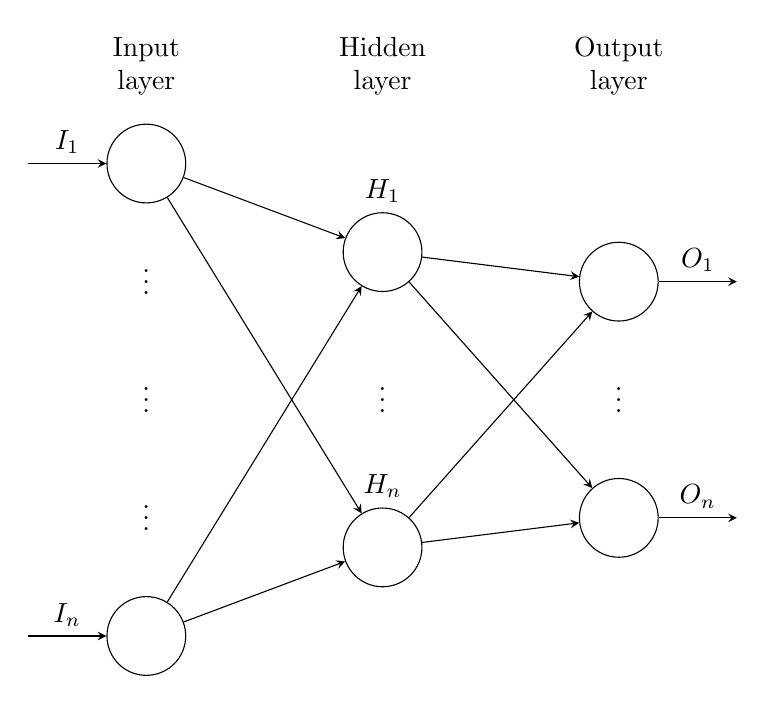
\begin{tikzpicture}[x=1.5cm, y=1.5cm, >=stealth]
			
			\foreach \m/\l [count=\y] in {1,missing, missing, missing, 5}
			\node [every neuron/.try, neuron \m/.try] (input-\y) at (0,2.5-\y) {};
			
			\foreach \m [count=\y] in {1,missing,2}
			\node [every neuron/.try, neuron \m/.try ] (hidden-\m) at (2,2-\y*1.25) {};
			
			\foreach \m [count=\y] in {1,missing,2}
			\node [every neuron/.try, neuron \m/.try ] (output-\m) at (4,1.5-\y) {};
			
			
			\draw [<-] (input-1) -- ++(-1,0)
			node [above, midway] {$I_1$};
			
			\draw [<-] (input-5) -- ++(-1,0)
			node [above, midway] {$I_n$};
			
			\foreach \l [count=\i] in {1,n}
			\node [above] at (hidden-\i.north) {$H_\l$};
			
			\foreach \l [count=\i] in {1,n}
			\draw [->] (output-\i) -- ++(1,0)
			node [above, midway] {$O_\l$};
			
			\foreach \i in {1,5}
			\foreach \j in {1,...,2}
			\draw [->] (input-\i) -- (hidden-\j);
			
			\foreach \i in {1,...,2}
			\foreach \j in {1,...,2}
			\draw [->] (hidden-\i) -- (output-\j);
			
			\foreach \l [count=\x from 0] in {Input, Hidden , Output}
			\node [align=center, above] at (\x*2,2) {\l \\ layer};
			
			\end{tikzpicture}
		\centering
		\caption{Structure of a simple multi layer perceptron with one hidden layer.}
		\label{fig:mlp}
	\end{figure}
	
	All neurons of one layer propagate their output to every neuron of the following layer via a weighted connection. This results in the weight matrix $\matr{w}$, which - connecting a layer with $n$ neurons to a layer with $m$ neurons - has a shape of $n\times m$. A single layer of the \markup{MLP} can be denoted as the linear transformation
	
	\begin{equation}
		f(\matr{x}) = \matr{w}\vec{x} + \vec{b} 
	\end{equation}
	
	
	
	Since the basic arithmetic operations in a neural network are still linear in nature, simple linear combinations of those basic operations will in turn also result in a linear transformation, rendering the combination useless. Hence additional nonlinearities have to be introduced in order to be able to predict nonlinear processes. 
	
	For this purpose, functions $\varphi$ are applied to the outputs of the network's layers, resulting in the filtered layer output $\varphi(f(\matr{x}))$.
	
	Since an \markup{MLP} consists of chained layers, each processing the output of its predecessor, the equation of a full network with n layers can be denoted:
	\begin{equation}
		\matr{y}(\matr{x_0}) = \varphi_n(f_n(... \varphi_2(f_2(\varphi_1(f_1(\matr{x}_0)))))) \,.
	\end{equation}
	
	\subsection{Activation Functions}
	
		When applied to sequential layers, the \textbf{threshold function} as it is used in the original equation for a single perceptron \ref{eq:rosenblatt-perceptron} is a simple way to introduce nonlinearities into the network. The threshold function is inspired by the findings of \cite{McCulloch1943} and only allows $0$ and $1$ as possible output values, essentially modeling the behavior of a synaptic connection between biological neurons. 
		
		With the threshold $\epsilon$ it is defined as
		\begin{equation}
		\label{eq:acti-sw}
		\varphi_{thresh}(x) = \left\{
		\begin{array}{ll}
		1\text{, if } x > \epsilon \\
		0 \text{ else}\\
		\end{array}
		\right.
		\end{equation}
		However because of its discontinuity around the origin, the step function is not differentiable. Since differentiabilty is desirable in machine learning scenarios, other activation functions are commonly used:
		
		\textbf{Sigmoid}
		With a variable slope parameter $a$, the sigmoid function is defined as
		\begin{equation}
		\varphi_{sigmoid}(x) = \frac{1}{1+\exp(-a \cdot x)}
		\end{equation}
		
		It is often used as a continuous approximation for the threshold function since its continuous differentiability makes it well suited for frequently used training procedures such as gradient descend.\\
		
		\begin{figure}[ht]
			\centering
			\begin{tikzpicture}
			\begin{axis}[
			domain=-200:200,
			xmin=-10, xmax=10,
			ymin=-1.5, ymax=1.5,
			samples=401,
			axis y line=center,
			axis x line=middle,
			]
			\addplot+[mark=none] {1/(1 + exp(-x)};
			\end{axis}
			\end{tikzpicture}
			\caption{Similar to the threshold function, the sigmoid function limits the output values to the interval [0, 1].}
			\label{fig:sigmoid_plot}
		\end{figure}
		
		
		\textbf{ReLU}
		The Rectifying Linear Unit (short: \markup{ReLU}\abbrev{ReLU}{Rectifying linear unit}) is an activation function which truncates any input value which is less than zero and is linear for positive inputs. Hence it can be defined as
		\begin{equation}
		\label{eq:relu_def}
		\varphi(x) = \max(x, 0)
		\end{equation}
		which truncates negative values. Compared to the threshold or sigmoid function, large input values do not lead to saturation (and thus to a vanishing gradient), which is particularly advantageous in gradient methods such as those described in section \ref{sec:gradient-descend}. Additionally, Glorot et. al. \cite{Glorot2011} state that by effectively zeroing hidden units, ReLU aids in establishing sparse representations which has advantages from both, a mathematical and from a biological plausibility point of view. Because of those advantages it is commonly used in feature extractors for computer vision tasks. \\
		
		\begin{figure}[ht]
			\centering
			\begin{tikzpicture}
			\begin{axis}[
			domain=-200:200,
			xmin=-10, xmax=10,
			ymin=-10, ymax=10,
			samples=401,
			axis y line=center,
			axis x line=middle,
			]
			\addplot+[mark=none] {max(x, 0)};
			\end{axis}
			\end{tikzpicture}
			\caption{Form of the ReLU activation function. Negative values are truncated.}
			\label{fig:relu_plot}
		\end{figure}
		
		Additionally, ReLu can be modified to be suitable for various applications. Two common modifications are leaky ReLU, denoted by 
		
		\begin{equation}
		\varphi_{ReLU_{leaky}} = \begin{cases}
		x \text{, if } x \geq 0 \\
		\alpha x \text{, if} x < 0
		\end{cases} \,,
		\end{equation} 
		which allows a scaled version of the layer's output to pass through and $\text{ReLU}n$ where $n$ denotes the maximum allowed output value for the given unit \cite{Sandler}:
		\begin{equation}
		\varphi_{ReLUn} = min(max(x, 0), n)
		\end{equation}
	
	
	\subsection { Convolutional Neural Networks (CNN) }
		Convolutional Neural Networks (\markup{CNN}\abbrev{CNN}{Convolutional Neural Network}), first introduced by Denker et al. in 1989 \cite{Denker1988} and improved by LeCun et al. \cite{LeCun1989} are a special case of neural networks that are particularly suitable for processing higher-dimensional structures such as images or temporal sequences of data since they are less prone to the curse of dimensionality.
		
		The input layer of a fully connected network requires one neuron for every pixel in every channel of the input, resulting in a quickly rising amount of weights if one of the image dimensions increases. A single depth map with dimensions of $224 \times 224$ pixels as it is used in this thesis would need 50176 neurons in the input layer alone, resulting in $50176 \cdot n$ ($n$ denoting the amount of neurons in the second layer) weights for the transition between the first two layers. 
		
		Convolutional Neural Networks solve this problem by having a fixed amount of weights in form of matrices which are moved over the inputs to perform convolutions.  
		
		
		
		
		
		In the case of a 2D CNN, the input data is a 2D matrix and each convolution layer also contains several two-dimensional matrices, which are moved over the input matrix to calculate the output data. 
		
		
		\todo{Bild für Faltung}
	
	
	\subsubsection { Recurrent Neural Networks (RNN) }
	
	\subsubsection { Long Short Term Memory (LSTM) }
	
	
		
\section { Machine Learning }
	\begin{displayquote}[{Russell, Norvig \cite{Russell2016}}]
		An agent is learning if it improves its performance on future tasks after making observations about the world.
	\end{displayquote}
	
	
	\subsection { Types of machine learning }

		The previous sections assumed the respective networks to be trained for their given task and hence having a predefined set of parameters. However, for real applications the parameters are not known beforehand and have to be learned by training the net on example data, defined by the set of $n$ observations $\mathbb{X} = \set{\matr{X_1},\matr{ X_2}, ..., \matr{X_n}}$ and (in some cases) the set of corresponding labels $\mathbb{Y} = \set{\matr{Y_1},\matr{Y_2}, ..., \matr{Y_n}}$. The objective during the learning process is to deduce a general model from a set of input data \cite{Bishop2009}. 
	
		
		Depending on the task to be performed, the example data can have different forms. For machine vision applications, the observed input has the form of an image
		
		Usually, a distinction is made between three forms of machine learning:
		
		\begin{itemize}
			\item Supervised learning solves the problem of finding a parameter set for tasks where observations and corresponding labels are given. 
			
			\item Unsupervised learning is the problem of learning a parameter set without any form of labels. This requires to learn the inherent structure of the input data through clustering or grouping of the input data.
			
			\item Semi-supervised learning uses strategies from supervised learning, as well as from unsupervised learning in combination in order to obtain improvements in learning accuracy. 
			

		\end{itemize}
	
		Generalization is an important objective in all machine learning tasks. 
		
		\subsection{Learning Algorithms}

		\subsubsection{Gradient Descend}
		\label{sec:gradient-descend}
		
		\subsubsection{ADAM}
		\todo{Link zum Paper ist in tensorflow source von adam optimizer zu finden}
		
	\subsection{ One Shot Learning }
	Ein Problem der bisher gezeigten Machine Learning-Methoden ist, dass sehr viele Traningsdaten benötigt werden, um die Netze ausreichend zu trainieren. In Anwendungsfällen, in denen die Trainingsdaten erst in der Benutzerinteraktion zur Verfügung stehen, können jedoch häufig nicht ausreichend viele Daten gesammelt werden. 
	
	Ein klassischer Anwendungsfall für One Shot learning ist daher zum Beispiel die Gesichtserkennung in Anwendersoftware. Hier muss es möglich sein, mit wenigen Gesichtern als Vorlage ein Gesicht auf einem neuen Photo zuverlässig wiederzuerkennen. Gleichzeitig sollte es jeder Zeit möglich sein, neue Klassen hinzuzufügen oder alte Klassen zu entfernen. Auch hier ist ein klassisches Netzwerk mit einer festen Anzahl von Ausgangsneuronen - und damit Klassen - ungeeignet.

	\subsubsection{Funktionsprinzip}
		Siamesische Netze sind eine mögliche Lösung für beide genannten Probleme: Sie vergleichen zwei Eingangstensoren und errechnen aus diesen einen Ähnlichkeitsfaktor. Anhand dieses Faktors kann nach Vergleich des unbekannten Eingangs mit allen bekannten Klassen diejenige mit der höchsten Übereinstimmung (oder keine im Fall eines Negativbeispiels) gewählt werden.
		
	\subsubsection{Aufbau des Netzes}
	 Bei einem Siamesischen Netzwerk handelt es sich um ein zweistufiges Netz, bestehend aus zwei Faltungsnetzen mit identischen Gewichten in der ersten Stufe, deren Ergebnis-Vektoren in der zweiten Stufe durch ein zusammenfassendes mehrlagiges Perzeptron in einen einzelnen Ähnlichkeits-Wert umgerechnet werden.
	 Die Faltungsnetze dienen dabei der Dimensionsreduktion - sie reduzieren den Eingangstensor auf einen Festure-Vektor und komprimieren damit die zur Verfügung stehende Information \todo{weiter}
	 
	 
	 
%	 \begin{figure}
%	 	\centering
%	 	 \newcommand*{\h}{\hspace{5pt}}% for indentation
 \newcommand*{\hh}{\h\h}% double indentation
  \begin{tikzpicture}[auto,
    %decision/.style={diamond, draw=black, thick, fill=white,
    %text width=8em, text badly centered,
    %inner sep=1pt, font=\sffamily\small},
    block_center/.style ={rectangle, draw=black, thick, fill=white,
      text width=8em, text centered,
      minimum height=4em},
    block_left/.style ={rectangle, draw=black, thick, fill=white,
      text width=16em, text ragged, minimum height=4em, inner sep=6pt},
    block_noborder/.style ={rectangle, draw=none, thick, fill=none,
      text width=18em, text centered, minimum height=1em},
    block_assign/.style ={rectangle, draw=black, thick, fill=white,
      text width=18em, text ragged, minimum height=3em, inner sep=6pt},
    block_lost/.style ={rectangle, draw=black, thick, fill=white,
      text width=16em, text ragged, minimum height=3em, inner sep=6pt},
      line/.style ={draw, thick, -latex', shorten >=0pt}]
    % outlining the flowchart using the PGF/TikZ matrix funtion
    \matrix [column sep=5mm,row sep=3mm] {
      % enrollment - row 1
      \node [block_center] (referred) {Referred (n=173)};
      & \node [block_left] (excluded1) {Excluded (n=17): \\
        a) Did not wish to participate (n=9) \\
        b) Did not show for interview (n=5) \\
        c) Other reasons (n=3)}; \\
      % enrollment - row 2
      \node [block_center] (assessment) {Assessed for eligibility (n=156)}; 
      & \node [block_left] (excluded2) {Excluded (n=54): \\
        a) Inclusion criteria not met (n=22) \\
        b) Exclusion criteria(s) met (n=13) \\
        c) Not suited for group (n=7) \\
        d) Not suited for CBT (n=2) \\
        e) Sought other treatment (n=3) \\
        f) Other reasons (n=7)}; \\
      % enrollment - row 3
      \node [block_center] (random) {Randomised (n=102)}; 
      & \\
      % follow-up - row 4
      \node [block_noborder] (i) {Intervention group}; 
      & \node [block_noborder] (wlc) {Wait-list control group}; \\
      % follow-up - row 5
      \node [block_assign] (i_T0) {Allocated to intervention (n=51): \\
      \h Received intervention (n=49) \\
      \h Did not receive intervention (n=2, \\
      \hh 1 with primary anxiety disorder, \\
      \hh 1 could not find time to participate)}; 
	  & \node [block_assign] (wlc_T0) {Allocated to wait-list (n=51): \\
      \h Stayed on wait-list (n=48) \\
      \h Did not stay on wait-list (n=3, \\
      \hh 2 changed jobs and lost motivation, \\
      \hh 1 was offered treatment elsewhere)}; \\
      % follow-up - row 6
      \node [block_lost] (i_T3) {Post-intervention measurement: \\
      \h Lost to follow-up (n=5, \\
      \hh 2 dropped out of the intervention, \\
      \hh 3 did not complete measurement)}; 
	  & \node [block_lost] (wlc_T3) {Post-wait-list measurement: \\
      \h Lost to follow-up (n=6, \\
      \hh 3 dropped out of the wait-list, \\
      \hh 3 did not complete measurement)}; \\
      % follow-up - row 7
      % empty first column for intervention group 
      & \node [block_assign] (wlc_T36) {Allocated to intervention (n=48): \\
      \h Received intervention (n=46) \\
      \h Did not receive intervention (n=2, \\
      \hh 1 reported low motivation, \\
      \hh 1 could not find time to participate)}; \\
      % follow-up - row 8
      \node [block_lost] (i_T6) {3-months follow-up measurement: \\
      \h Lost to follow-up (n=9, \\
      \hh did not complete measurement)}; 
      & \node [block_lost] (wlc_T6) {Post-intervention measurement: \\
      \h Lost to follow-up (n=5, \\
      \hh 2 dropped out of the intervention, \\
      \hh 3 did not complete measurement)}; \\
      % follow-up - row 9
      % empty first column for intervention group 
      & \node [block_lost] (wlc_T9) {3-months follow-up measurement \\
      \h Lost to follow-up (n=2, \\
      \hh did not complete measurement)}; \\
      % analysis - row 10
      \node [block_assign] (i_ana) {Analysed (n=51)}; 
      & \node [block_assign] (wlc_ana) {Analysed (n=51)}; \\
    };% end matrix
    % connecting nodes with paths
    \begin{scope}[every path/.style=line]
      % paths for enrollemnt rows
      \path (referred)   -- (excluded1);
      \path (referred)   -- (assessment);
      \path (assessment) -- (excluded2);
      \path (assessment) -- (random);
      \path (random)     -- (i);
      \path (random)     -| (wlc);
      % paths for i-group follow-up rows
      \path (i)          -- (i_T0);
      \path (i_T0)       -- (i_T3);
      \path (i_T3)       -- (i_T6);
      \path (i_T6)       -- (i_ana);
      % paths for wlc-group follow-up rows
      \path (wlc)        -- (wlc_T0);
      \path (wlc_T0)     -- (wlc_T3);
      \path (wlc_T3)     -- (wlc_T36);
      \path (wlc_T36)    -- (wlc_T6);
      \path (wlc_T6)     -- (wlc_T9);
      \path (wlc_T9)     -- (wlc_ana);
    \end{scope}
  \end{tikzpicture}

%	 	\caption{Aufbau eines siamesischen Netzwerkes}
%	 	\label{fig:siamesenetwork}
%	 \end{figure}
	 
	 	 \subsubsection{Triplet Loss}
	 Da das Netzwerk \todo{weiter}
	 
	 
	 
	 Hierfür kann ein Siamesisches Netzwerk (en.: siamese network) genutzt werden. 

		\subsection{Nearest Neighbors}
	(k-)Nearest Neighbor (\markup{k-NN}\abbrev{k-NN}{k-Nearest Neighbors}) algorithms as described in \cite{Cover1967, Fix1952} are based on the assumption that samples which are close in a (appropriate) metric will belong to the same class. Hence they provide a simple decision rule for classification problems where no underlying distribution of the sample points is known. 
	
	Given a set of training vectors in a multidimensional feature space, each with their corresponding class label, the k-NN algorithm uses majority-voting among $k$ of the closest examples from the training data to determine the class of a new, unknown example.
	
	A common distance metric for k-NN is the euclidean distance but depending on the structure of the data to be classified, other distance metrics (like the Hamming Distance for texts) may be used.
	
	With growing size of the example pool, naive implementations of k-NN become too computationally intensive since for every test point $t$, the distance to every available training sample has to be calculated. This effect can be reduced by pre-partitioning the training data in such a way that parts of it can be ignored when classifying a new sample. 
	
	One example for this kind of pre-partitioning is the \textit{Ball Tree} or \textit{Metric Tree} which is generated by recursively dividing the feature set into subgroups, thus generating a binary tree. The descendants of a parent node are calculated such that the division causes the maximum spread along a single feature dimension. This is useful for \markup{k-NN} since child nodes (and thus all their children) which have a higher distance to the test point $t$ than the current best candidates can be ignored, potentially saving many comparisons for high-dimensional features.
	
	\begin{figure}
		\centering
		\fontsize{7.5pt}{11pt}\selectfont% or whatever fontsize you like
		\begin{subfigure}[c]{0.4\textwidth}
			\centering
			\def\svgwidth{\textwidth}
			\input{Ressourcen/ball-tree-2d.pdf_tex}
			\subcaption{Subfigure Bild Nr. 1}
		\end{subfigure}
		\begin{subfigure}[c]{0.4\textwidth}
			\centering
			\def\svgwidth{\textwidth}
			\input{Ressourcen/ball-tree-graph.pdf_tex}
			\subcaption{Subfigure Bild Nr. 1}
		\end{subfigure}
		\caption{}
		\label{fig:simpleperceptron}
	\end{figure}
	
	
\section { Modeling the human hand }
	\abbrev{PIP}{Proximal Interphalangeal, see Figure \ref{fig:malik2018handmodel}}
	\abbrev{DIP}{Distal Interphalangeal, see Figure \ref{fig:malik2018handmodel}}
	\abbrev{MCP}{Metacarpophalangeal, see Figure \ref{fig:malik2018handmodel}}
	\abbrev{TIP}{Finger Tip}
	
	\begin{figure}
		\centering
		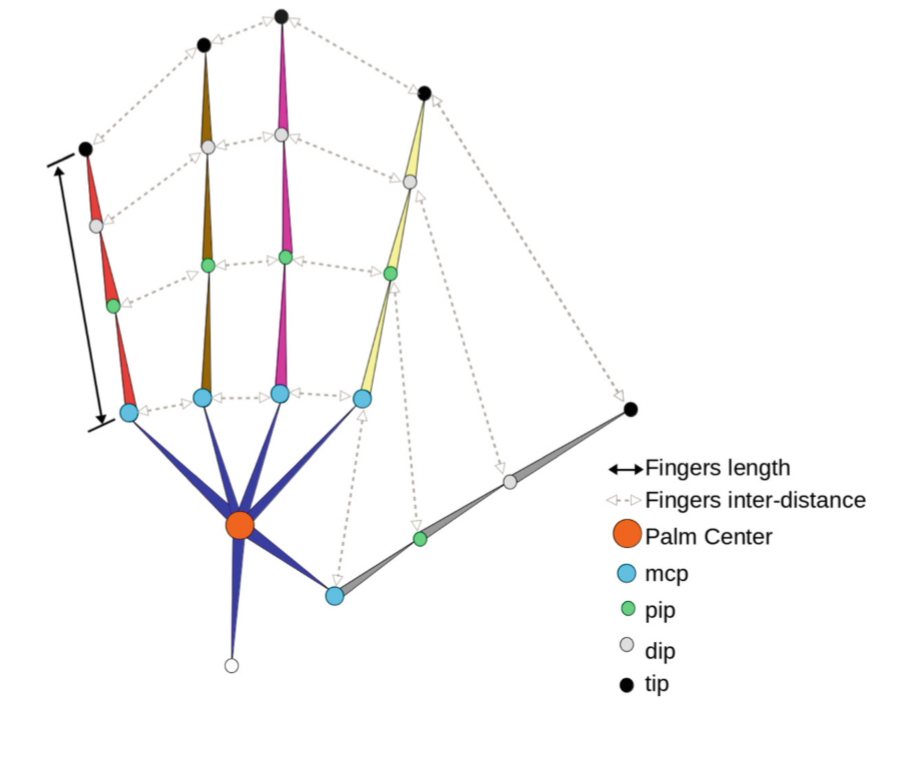
\includegraphics[width=0.7\linewidth]{Ressourcen/malik2018_hand_model}
		\caption[Handmodell nach \cite{Malik2018b}]{In \cite{Malik2018b} wird ein Modell ähnlich dem oben stehenden (Quelle: \cite{Malik2018b}) genutzt, in dem die vollständige Handpose durch 21, bzw. 22 (Gelenk-) Koordinaten bestimmt ist.}
		\label{fig:malik2018handmodel}
	\end{figure}
	Throughout this thesis, the hand model shown in Figure \ref{fig:malik2018handmodel} will be used as it provides enough key points to reconstruct hand poses to a sufficient degree.
	
	The freedom of movement of the individual joints of the hand is subject to anatomical restrictions. Modeling those restrictions can be useful to assess the quality of the estimate and to refine it accordingly. In \cite{Lin2000} the main constraints are divided into two types: 
	
	Type 1 constraints describe the valid flexion and abduction/adduction angles
	
	\begin{alignat}{7}
		&&0\degree \quad &&\leq \quad &&\theta_{MCP_F} \quad &&\leq \quad &90\degree\, &&,\\
		&&0\degree \quad &&\leq \quad &&\theta_{PIP_F} \quad &&\leq \quad &110\degree\,&& ,\\
		&&0\degree \quad &&\leq \quad &&\theta_{DIP_F} \quad &&\leq \quad &90\degree\, && \text{and}\\
		&&-15\degree \quad &&\leq \quad &&\theta_{MCP_AA} \quad &&\leq \quad &15\degree\, &&,
	\end{alignat}
	
	\begin{equation}
	\theta_{MCP_AA} = 0\degree\, \text{and}
	\end{equation}

	\begin{equation}
	\theta_{TM_AA} = 0\degree\,.
	\end{equation}
	
	Type 2 constraints describe inter- and intra finger limits in motion:
	A natural motion of the proximal interphalangeal (\markup{PIP}) will cause a proportional motion in the corresponding distal interphalangeal (\markup{DIP}).
	
	This relation can be denoted as 
	\begin{equation}
	\theta_{DIP} = \frac{2}{3}\theta_{PIP}\,.
	\end{equation}
	
	
\section{Kameraparameter}
\subsection{Intrinsische Parameter}
Die intrinsischen Paramter einer Kamera sind definiert durch die Brennweite $f$, das Format des Bildsensors und 
\subsection{Extrinsische Parameter}

\section{YOLO}
\markup{YOLO}\abbrev{YOLO}{You Only Look Once - Object detection Network} is a convolutional object detection network, described in \cite{Redmon2016}. Which uses an architecture similar to GoogLeNet \cite{Szegedy2014}. Instead of inception modules, as used in GoogLeNet, \cite{Redmon2016} uses building blocks with $1\times1$ reduction layers, followed by $3\times3$ convolutional layers. 

\begin{figure}[ht]
	\centering
	\includegraphics[width=0.7\linewidth]{Ressourcen/yolo-net}
	\caption[Architecture of the YOLO network.]{Architecture of the YOLO network. Source: \cite{Redmon2016}}
	\label{fig:yolo-net}
\end{figure}


	